

\section{Full details of the Simple Protocol Example}

\label{Appendix:FullExample}


%% \begin{figure}[t]
%%    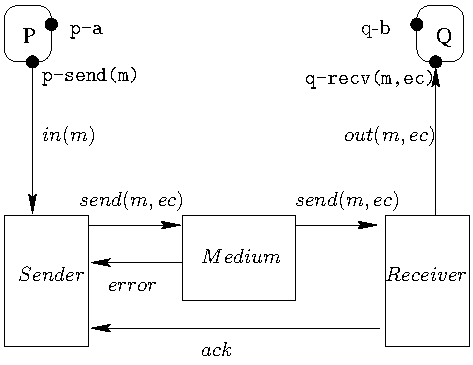
\includegraphics[width=5.5cm]{XFIG/SimpleProt-Schema}
%%    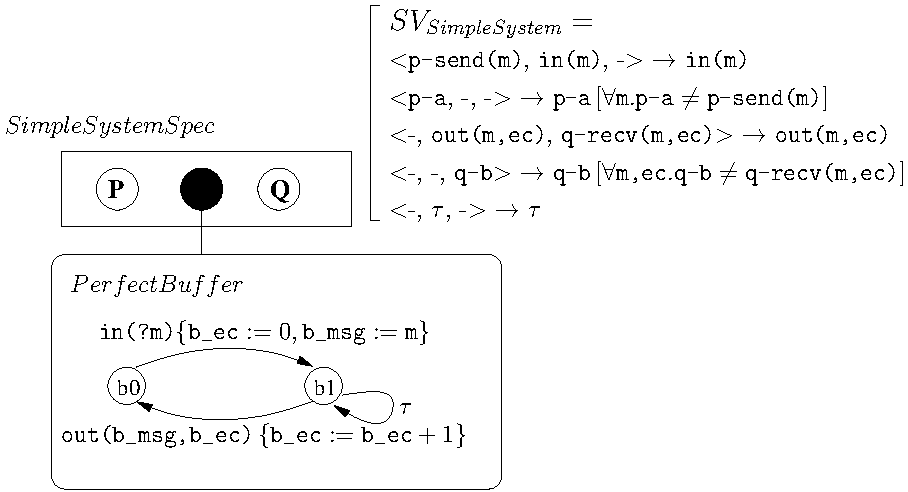
\includegraphics[width=6.5cm]{XFIG/SimpleProt2-Spec}
%%    \caption{Specification pNet Schema and Specification}
%%    \label{App:SimpleProt:Spec}

%% \end{figure}

  
%% \begin{figure}[t]
%%   \centerline{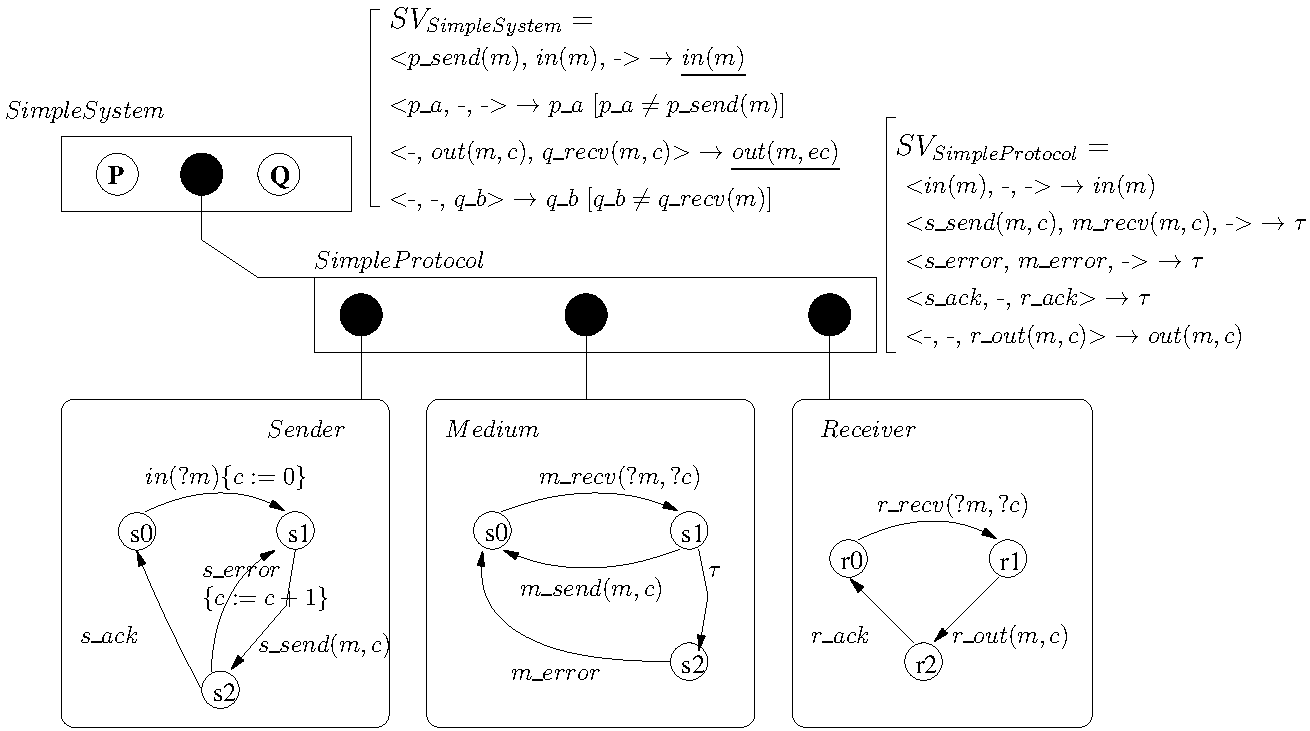
\includegraphics[width=12cm]{XFIG/SimpleProt2-pNet}}
%%   \caption{Composed pNet with the Simple Protocol Implementation}  \label{App:SimpleProt:Impl}
%% \end{figure}

The first piece of code is the textual definition of the SimpleProtSec
pNet, that was drawn in Figure \ref{SimpleProt:Impl}, page \pageref{SimpleProt:Impl}. This code should be intuitive enough to read, with the following
conventions, that brings some user-friendly features that are maps by the editor into pure pNet constructs.

\begin{itemize}
  \item Constants of any type (including Action) must be declared as
    ``const''. They are used either as functions with argument, as
    typically \texttt{in(msg)}, or constants without argument, denoted
    as \texttt{\$tau}. Identifiers without the ``?'' marker are
    variables.
  \item Variables can be declared either: inside a pLTS state (normal
    state variable), as global variable of a pLTS (see e.g. ...), or
    as an input variable in a transition, as \texttt{?msg} in pLTS M1
    here.
  \item the variables in the guards of synchronisation vectors do not need to be explicitely quantified: all variable in a guard that does not appear inside the vector actions will be recognised as bound by a \emph{foral} quantifier inside the guard.
    \item the tools will check that everything is correctly declared, and that variables are used properly, that vectors have coherent length, etc.
\end{itemize}

\TODO{Je ne peux pas refaire tourner le code, il faut que je modifie le pNet Editor pour qu'ils n'utilise plus les variables d'etat... Donc les 3 prochaines pages sont obsoletes...}
%% \TODO{keep ?}
%% \paragraph{Variable management.}
%% The variables in each synchronisation vector are considered local:
%% for a given pNet expression, we must have fresh local variables for
%% each occurrence of a vector (i.e. each time we instantiate rule
%% \TrDeux). Similarly the state variables of each copy of a
%% given pLTS in the system, must be distinct, and those created for each
%% application of \TrDeux\ have to be fresh and all distinct. 
%% This is implemented within the open-automaton generation algorithm,
%% using name generation using a global counter as a suffix.

\begin{lstlisting}[basicstyle=\scriptsize\ttfamily, language=java, frame=single]
SimpleProtSpec2:
import "Data_Alg.algp"
root SimpleProtSpec2
const in, out:Action
const p_send, q_recv: Action
const tau:Action

pLTS M1
initial a0 
vars ?msg:Data

state a0
transition in(msg) -> a1 {a1_msg:=msg, m1_ec:=0}

state a1
vars a1_msg:Data m1_ec:Int
transition out(a1_msg, m1_ec) -> a0
transition synchro($tau)  -> a1 {m1_ec:=m1_ec+1}

pNet SimpleProtSpec2
holes P,Q
subnets P,M1,Q
vars p_a,q_a:Action m:Data ec:Int

vector SV0 <p_send(m), in(m),_>->synchro(in(m))
vector SV1 <p_a,_,_>->p_a [p_a != p_send(m)]
vector SV2 <_, out(m,ec), q_recv(m)>->synchro(out(m,ec))
vector SV3 <_,_,q_a>->q_a [q_a != q_recv(m)]

  \end{lstlisting}

The corresponding generated Open Automaton was given in Figure \ref{SimpleProtCounter:SpecOA},
page \pageref{SimpleProtCounter:SpecOA}.

Next is the code for the SimpleProtImpl pNet:

\begin{lstlisting}[basicstyle=\scriptsize\ttfamily, language=java, frame=single]
SimpleProtImpl2:
import "Data_Alg.algp"
root SimpleProtImpl2

const in,out:Action
const tau,p_send,q_recv,m_recv,m_send,m_error: Action
const s_recv,s_send,s_ack,s_error,r_recv,r_ack,r_send: Action

pLTS M1
  initial a0
  vars ?msg:Data ?c:Int

state a0
transition m_recv(msg,c) -> a1 {a1_msg:=msg, a1_ec:=c}

state a1
vars a1_msg:Data a1_ec:Int
transition m_send(a1_msg, a1_ec) -> a0 
transition synchro($tau) -> a2

state a2
transition $m_error -> a0

pLTS Sender
  initial s0
  vars ?msg:Data

state s0
transition s_recv(msg) -> s1 {s1_msg:=msg, s1_ec:=0}

state s1
vars s1_msg:Data s1_ec:Int
transition s_send(s1_msg, s1_ec) -> s2 {s2_ec:=s1_ec}

state s2
vars  s2_ec:Int
transition $s_ack -> s0
transition $s_error -> s1 {s1_ec:=s2_ec+1}

pLTS Receiver
  initial r0
  vars ?msg:Data ?c:Int

state r0
transition r_recv(msg,c) -> r1 {r1_msg:=msg, r1_ec:=c}

state r1
vars r1_msg:Data r1_ec:Int
transition r_send(r1_msg, r1_ec) -> r2

state r2
transition $r_ack -> r0

pNet medium
  subnets Sender, M1, Receiver
  vars m:Data c:Int
vector SV0 <s_recv(m), _, _>->in(m)
vector SV1 <s_send(m,c), m_recv(m,c), _>->synchro($tau)
vector SV2 <_, m_send(m,c), r_recv(m,c)>->synchro($tau)
vector SV3 <$s_ack, _, $r_ack>->synchro($tau)
vector SV4 <$s_error, $m_error, _>->synchro($tau)
vector SV5 <_, _, r_send(m,c)>->out(m,c)

pNet SimpleProtImpl2
  holes P,Q
  subnets P,medium,Q
  vars p_a,q_a:Action  m:Data c:Int
vector SV0 <p_send(m), in(m),_>->synchro(in(m))
vector SV1 <p_a,_,_>->p_a [p_a != p_send(m)]
vector SV2 <_, out(m,c), q_recv(m,c)>->synchro(out(m,c))
vector SV3 <_,_,q_a>->q_a [q_a != q_recv(m,c)]
\end{lstlisting}

%% From this code,A more compact view (maybe more readable ???) is given
%% by the pretty-printer of VerCors:

%% \begin{lstlisting}[basicstyle=\scriptsize\ttfamily, language=java, frame=single]
%% SimpleProtImpl2
%% --------------------
%% SV6 SVs: <p_send(m), in(m), _>-->in(m)
%% SV7 SVs: <p_a, _, _>-->p_a, p_a!=(p_send(m))
%% SV8 SVs: <_, out(m, c), q_recv(m, c)>-->out(m, c)
%% SV9 SVs: <_, _, q_a>-->q_a, q_a!=(q_recv(m, c))
%% SV11 SVs: <_, _tau_, _>-->_tau_
%% Holes: P
%% Subnets: medium
%% - medium
%% - SV0 SVs: <in(m), _, _>-->in(m)
%% - SV1 SVs: <s_send(m, c), m_recv(m, c), _>-->_tau_
%% - SV2 SVs: <_, m_send(m), r_recv(m)>-->_tau_
%% - SV3 SVs: <s_ack, _, r_ack>-->_tau_
%% - SV4 SVs: <s_error, m_error, _>-->_tau_
%% - SV5 SVs: <_, _, out(m, c)>-->out(m, c)
%% - SV10 SVs: <_, _tau_, _>-->_tau_
%% - pLTS: Sender
%% - - Transition: s0---in(msg)-->s1, { s1_msg := msg s1_ec := 0}
%% - - Transition: s1---s_send(s1_msg, s1_ec)-->s2, {}
%% - - Transition: s2---s_ack-->s0, {}
%% - - Transition: s2---s_error-->s1, { s1_ec := s2_ec+1}
%% - - Variable: s1_ec, State: s1, Value(s) = 0,s2_ec+1,
%% - - Variable: s1_msg, State: s1, Value(s) = msg,
%% - pLTS: M1
%% - - Transition: a0---m_recv(msg, c)-->a1, { a1_msg := msg a1_ec := c}
%% - - Transition: a1---m_send(a1_msg, a1_ec)-->a0, {}
%% - - Transition: a1---_tau_-->a2, {}
%% - - Transition: a2---m_error-->a0, {}
%% - - Variable: a1_msg, State: a1, Value(s) = msg,
%% - - Variable: a1_ec, State: a1, Value(s) = c,
%% - pLTS: Receiver
%% - - Transition: r0---r_recv(msg, c)-->r1, { r1_msg := msg r1_ec := c}
%% - - Transition: r1---out(r1_msg, r1_ec)-->r2, {}
%% - - Transition: r2---r_ack-->r0, {}
%% - - Variable: r1_msg, State: r1, Value(s) = msg,
%% - - Variable: r1_ec, State: r1, Value(s) = c,
%% Holes: Q
%% \end{lstlisting}

Finaly, we list here in raw format, the 19 OTs computed by the tool for the SimpleProtImpl pNet.
This view uses variable names very close to the internal representation in the tool, allowing for traceability of generated fresh variables. For example:
\begin{itemize}
\item m:SV6:1:1 refers to a variable named ``m'' in the synchronisation vector ``SV6''; the last 2 numbers allows to distinguish different clones.
\item the other variable names reflect our naming policy: state variables are prefixed by the name of the state, holes actions by the name of the hole.
\end{itemize}

\TODO{To be updated completely}

\begin{lstlisting}[basicstyle=\scriptsize\ttfamily, language=java, frame=single]

{P|->p_send(m:SV6:1:1)},
[(msg=m:SV0:12:1)/\((s_recv(msg))=(s_recv(m:SV0:12:1)))], {s1_msg := msg, s1_ec := 0}
	OT:1 ------------------------------------------------------------
		<s0_a0_r0>-----_in(m:SV6:1:1)_----><s1_a0_r0>

{P|->p_a:SV7:1:2},
[(forall:m:SV7:1:2. (p_a:SV7:1:2!=(p_send(m:SV7:1:2)))], {}
	OT:2 ------------------------------------------------------------
		<s0_a0_r0>-----p_a:SV7:1:2----><s0_a0_r0>

{Q|->q_a:SV9:1:4},
[(forall:m:SV9:1:4,c:SV9:1:4. (q_a:SV9:1:4!=(q_recv(m:SV9:1:4, c:SV9:1:4)))],   {}
	OT:3 ------------------------------------------------------------
		<s0_a0_r0>-----q_a:SV9:1:4----><s0_a0_r0>

INFO  SimpleProtImpl2 - 
{P|->p_a:SV7:1:2},
[(forall:m:SV7:1:2. (p_a:SV7:1:2!=(p_send(m:SV7:1:2)))],   {}
	OT:4 ------------------------------------------------------------
		<s1_a0_r0>-----p_a:SV7:1:2----><s1_a0_r0>

{Q|->q_a:SV9:1:4},
[(forall:m:SV9:1:4,c:SV9:1:4. (q_a:SV9:1:4!=(q_recv(m:SV9:1:4, c:SV9:1:4)))],   {}
	OT:5 ------------------------------------------------------------
		<s1_a0_r0>-----q_a:SV9:1:4----><s1_a0_r0>

{},   [(s1_msg=m:SV1:114:2)/\(s1_ec=c:SV1:114:2)
  /\((s_send(s1_msg, s1_ec))=(s_send(m:SV1:114:2, c:SV1:114:2)))
  /\(msg=m:SV1:114:2)/\(c=c:SV1:114:2)
  /\((m_recv(msg, c))=(m_recv(m:SV1:114:2, c:SV1:114:2)))],
{s2_ec := s1_ec, a1_msg := msg, a1_ec := c}
	OT:6 ------------------------------------------------------------
		<s1_a0_r0>-----_tau_----><s2_a1_r0>

{P|->p_a:SV7:1:2},
[(forall:m:SV7:1:2. (p_a:SV7:1:2!=(p_send(m:SV7:1:2)))],   {}
	OT:7 ------------------------------------------------------------
		<s2_a1_r0>-----p_a:SV7:1:2----><s2_a1_r0>

{Q|->q_a:SV9:1:4},
[(forall:m:SV9:1:4,c:SV9:1:4. (q_a:SV9:1:4!=(q_recv(m:SV9:1:4, c:SV9:1:4)))],   {}
	OT:8 ------------------------------------------------------------
		<s2_a1_r0>-----q_a:SV9:1:4----><s2_a1_r0>

{},   [(a1_msg=m:SV2:114:3)/\(a1_ec=c:SV2:114:3)
  /\((m_send(a1_msg, a1_ec))=(m_send(m:SV2:114:3, c:SV2:114:3)))
  /\(msg=m:SV2:114:3)/\(c=c:SV2:114:3)
  /\((r_recv(msg, c))=(r_recv(m:SV2:114:3, c:SV2:114:3)))],
{r1_msg := msg, r1_ec := c}
	OT:9 ------------------------------------------------------------
		<s2_a1_r0>-----_tau_----><s2_a0_r1>

		{},   [],   {}
	OT:10 ------------------------
		<s2_a1_r0>-----_tau_----><s2_a2_r0>

{P|->p_a:SV7:1:2},
[(forall:m:SV7:1:2. (p_a:SV7:1:2!=(p_send(m:SV7:1:2)))],   {}
	OT:11 ------------------------------------------------------------
		<s2_a0_r1>-----p_a:SV7:1:2----><s2_a0_r1>

{Q|->q_recv(m:SV8:1:3, c:SV8:1:3)},
[(r1_msg=m:SV5:18:6)/\(r1_ec=c:SV5:18:6)
  /\((r_send(r1_msg, r1_ec))=(r_send(m:SV5:18:6, c:SV5:18:6)))],   {}
	OT:12 ------------------------------------------------------------
		<s2_a0_r1>-----_out(m:SV8:1:3, c:SV8:1:3)_----><s2_a0_r2>

{Q|->q_a:SV9:1:4},
[(forall:m:SV9:1:4,c:SV9:1:4. (q_a:SV9:1:4!=(q_recv(m:SV9:1:4, c:SV9:1:4)))],   {}
	OT:13 ------------------------------------------------------------
		<s2_a0_r1>-----q_a:SV9:1:4----><s2_a0_r1>

{P|->p_a:SV7:1:2},
[(forall:m:SV7:1:2. (p_a:SV7:1:2!=(p_send(m:SV7:1:2)))],   {}
	OT:14 ------------------------------------------------------------
		<s2_a2_r0>-----p_a:SV7:1:2----><s2_a2_r0>

{Q|->q_a:SV9:1:4},
[(forall:m:SV9:1:4,c:SV9:1:4. (q_a:SV9:1:4!=(q_recv(m:SV9:1:4, c:SV9:1:4)))],   {}
	OT:15 ------------------------------------------------------------
		<s2_a2_r0>-----q_a:SV9:1:4----><s2_a2_r0>

		{},   [],   {s1_ec := s2_ec+1}
	OT:16 --------------------------------------
		<s2_a2_r0>-----_tau_----><s1_a0_r0>

{P|->p_a:SV7:1:2},
[(forall:m:SV7:1:2. (p_a:SV7:1:2!=(p_send(m:SV7:1:2)))],   {}
	OT:17 ------------------------------------------------------------
		<s2_a0_r2>-----p_a:SV7:1:2----><s2_a0_r2>

{Q|->q_a:SV9:1:4},
[(forall:m:SV9:1:4,c:SV9:1:4. (q_a:SV9:1:4!=(q_recv(m:SV9:1:4, c:SV9:1:4)))],   {}
	OT:18 ------------------------------------------------------------
		<s2_a0_r2>-----q_a:SV9:1:4----><s2_a0_r2>

		{},   [],   {}
	OT:19 ------------------------
		<s2_a0_r2>-----_tau_----><s0_a0_r0>


Assignements of state variables:

Global State: <s0_a0_r0>
===================
pLTS States: <s0 vars: {}> <a0 vars: {}> <r0 vars: {}>

Global State: <s1_a0_r0>
===================
pLTS States: <s1 vars: { s1_msg <-{msg} s1_ec <-{0, s2_ec+1}}> <a0 vars: {}> <r0 vars: {}>

Global State: <s2_a1_r0>
===================
pLTS States: <s2 vars: { s2_ec <-{s1_ec}}> <a1 vars: { a1_msg <-{msg} a1_ec <-{c}}> <r0 vars: {}>

Global State: <s2_a0_r1>
===================
pLTS States: <s2 vars: { s2_ec <-{s1_ec}}> <a0 vars: {}> <r1 vars: { r1_ec <-{c} r1_msg <-{msg}}>

Global State: <s2_a2_r0>
===================
pLTS States: <s2 vars: { s2_ec <-{s1_ec}}> <a2 vars: {}> <r0 vars: {}>

Global State: <s2_a0_r2>
===================
pLTS States: <s2 vars: { s2_ec <-{s1_ec}}> <a0 vars: {}> <r2 vars: {}>

INFO  SimpleProtImpl2 - Total: 19 SATISFIABLE OTs
INFO  SimpleProtImpl2 -        185 UNSATISFIABLE OTs
INFO  SimpleProtImpl2 - Total Time: 1105 ms

\end{lstlisting}

%% And here is a  drawing of this open automaton, slightly simplified for readability:

%% \begin{figure}[h]
%%   \centerline{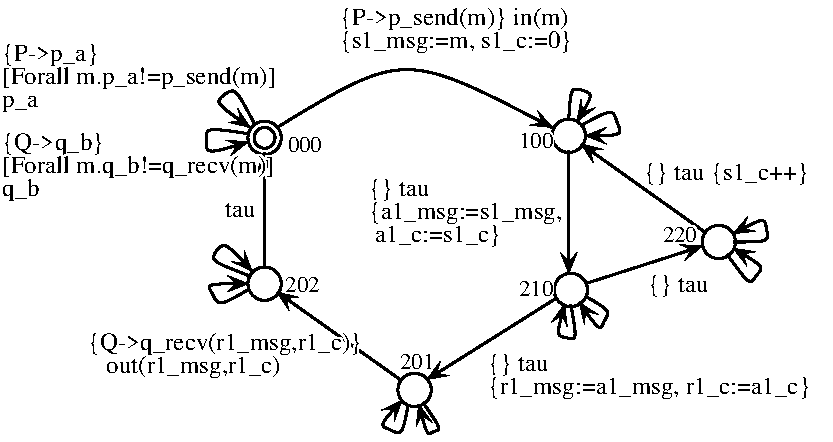
\includegraphics[width=10cm]{ATG/SPImplOpen}}
%%   \caption{Open Automaton of the Simple Protocol Implementation}  \label{Annex:SimpleProtCounter:ImplOA}
%% \end{figure}

%% And a partially saturated Automaton:

%% \begin{figure}[h]
%%   \centerline{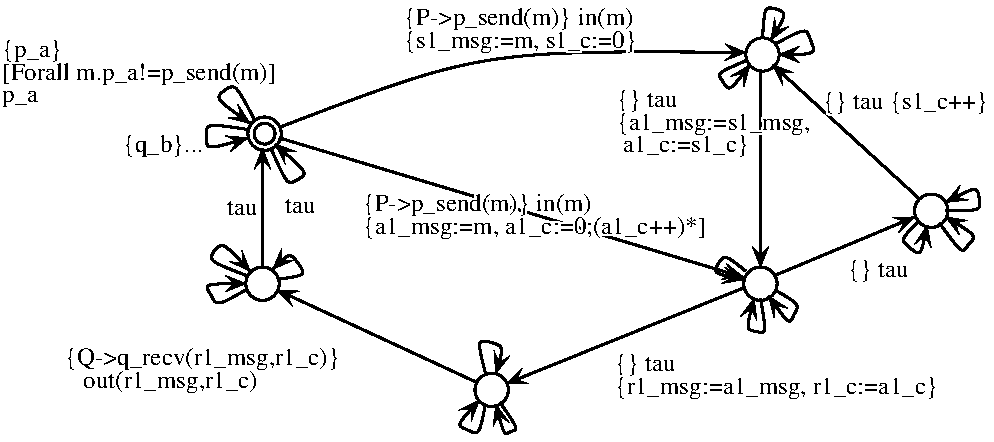
\includegraphics[width=13cm]{ATG/SPImplWeakOpen}}
%%   \caption{Weak Open Automaton, partial}  \label{SimpleProtCounter:ImplWOA}
%% \end{figure}

%% In Figure \ref{Annex:SimpleProtCounter:ImplWOA}, we have added some of the weak transitions generated by the saturation, namely:
%% - a tau-loop on each state
%% - a transition from <s0\_a0\_r0> to <s\_a\_r0>, resulting from the sequence OT\-1;OT\-6 followed by any number of the loop (OT\_9;ot\_12;OT\_6).
%%
%%Many weak should be added, e.g. Tau loops on states <s\_a\_r0>, <s\_a\_r0>, 
%%<s\_a0\_r0>, encoding the loop.

\begin{figure}[h]
   \centerline{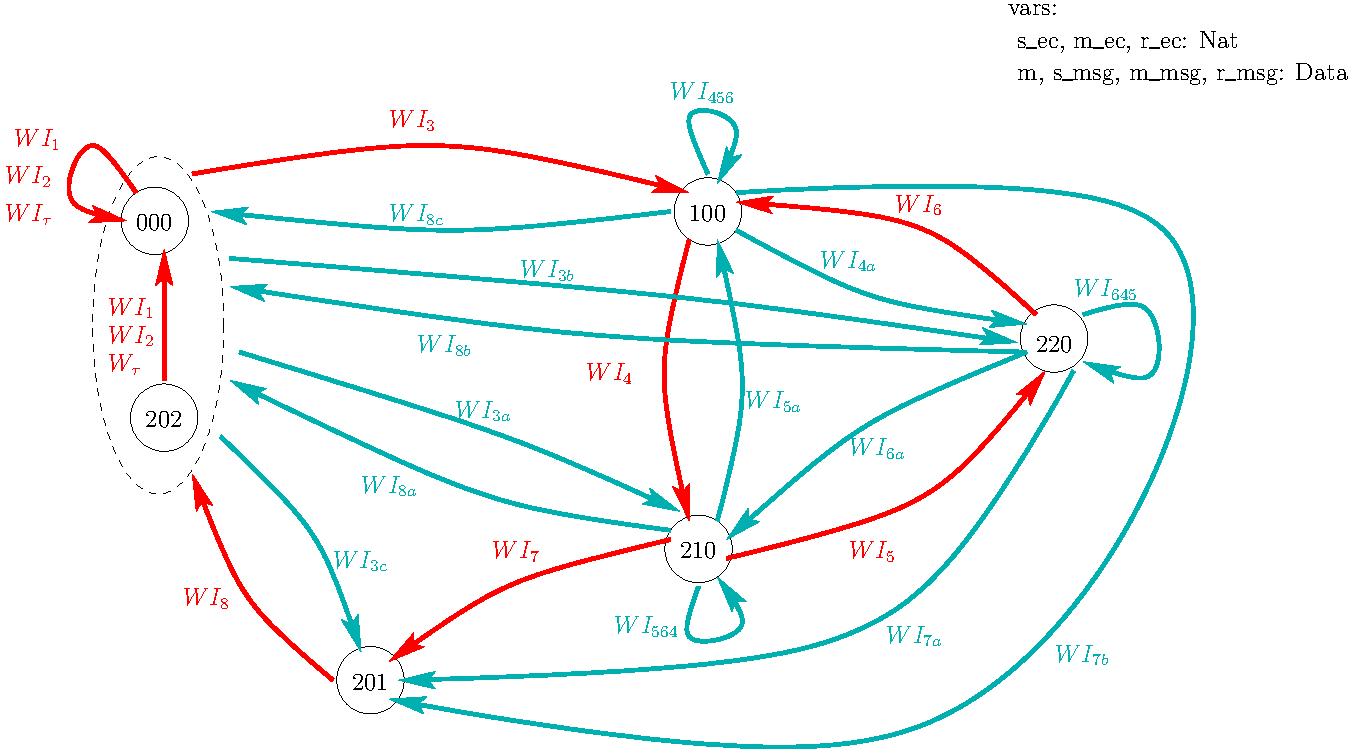
\includegraphics[width=10cm]{XFIG/SimpleProtImpl-WOA2}}
   \caption{Weak Open Automaton of the implementation}
   \label{Appendix:ImplOA2}
 \end{figure}

In Figure \ref{Appendix:ImplOA2} we recall the weak open automaton of our implementation pNet. 

It is based on the observation that states 202 and 000 are only linked by a "pure $\tau$" transition, and have exactly the same possible behaviours.
More tricky, they do not have the same state variables, as 202 has the variables of state $s2$, but none of these variables are used in transitions from 202.
In this configuration we can guarantee that they are Weak bisimilar, and merge their (incoming and outgoing) transitions in the Figure. We denote this 
equivalence class of states as $\{000,202\}$.
\TODO{May be express this property more formerly, but this could be also part of another paper, more oriented towards algorithms and optimisation of the Weak}


Details of the weak transitions is listed here:

In the first 3 weak transitions, $S$ denotes the set of all global states.

$ W_\tau = \openrule
{\{\}, True, ()}
{S \OTWeakarrow {\tau} S}$

$ WI_1 = \openrule
{\{\texttt{P}\mapsto \texttt{p-a}\}, [\forall \texttt{m}. \texttt{p-a} \neq \texttt{p-send(m)} ], ()}
{S \OTWeakarrow {\texttt{p-a}} S}$

$ WI_2 = \openrule
{\{\texttt{Q}\mapsto \texttt{q-b}\}, [\forall \texttt{m,ec}. \texttt{q-b} \neq \texttt{q-recv(m,ec)} ], ()}
{S \OTWeakarrow {\texttt{q-b}} S}$

All following transitions are parametrized by an arbitrary non-negative integer $n\in \mathcal{N}$.


$ WI_3(n) = \openrule
  {\{\texttt{P}\mapsto \texttt{p-send(m)}\}, True,
    (\texttt{s\_msg}\gets \texttt{m}, \texttt{s\_ec}\gets n)}
  { \{000,202\} \OTWeakarrow {\nounderline{\texttt{in(m)}}} 100}
$

$ WI_{3a}(n) = \openrule
  {\{\texttt{P}\mapsto \texttt{p-send(m)}\}, True,
    (\texttt{m\_msg}\gets \texttt{m}, \texttt{m\_ec}\gets n, \texttt{s\_ec}\gets n)}
  { \{000,202\} \OTWeakarrow {\nounderline{\texttt{in(m)}}} 210}
$

$ WI_{3b}(n) = \openrule
  {\{\texttt{P}\mapsto \texttt{p-send(m)}\}, True,
    (\texttt{s\_ec}\gets n)}
  { \{000,202\} \OTWeakarrow {\nounderline{\texttt{in(m)}}} 220}
$

$ WI_{3c}(n) = \openrule
  {\{\texttt{P}\mapsto \texttt{p-send(m)}\}, True,
    (\texttt{r\_msg}\gets \texttt{m}, \texttt{r\_ec}\gets n)}
  { \{000,202\} \OTWeakarrow {\nounderline{\texttt{in(m)}}} 201}
$

$ WI_4(n) = \openrule
         {\{\}, True, 
   (\texttt{m\_msg}\gets \texttt{s\_msg}, \texttt{m\_ec}\gets \texttt{s\_ec}+n, \texttt{s\_ec}\gets \texttt{s\_ec}+n)}
         {100 \OTWeakarrow {\tau} 210}
$

$ WI_{4a}(n) = \openrule
         {\{\}, True, 
    (\texttt{s\_ec}\gets \texttt{s\_ec}+n)}
         {100 \OTWeakarrow {\tau} 220}
$

$ WI_5(n) = \openrule
         {\{\}, True, (\texttt{s\_ec}\gets \texttt{s\_ec}+n)}
         {210 \OTWeakarrow {\tau} 220}
         \ \forall n\ge 0$

$ WI_{5a}(n) = \openrule
         {\{\}, True, (\texttt{s\_ec}\gets \texttt{s\_ec}+1+n)}
         {210 \OTWeakarrow {\tau} 100}
         \ \forall n\ge 0$


$ WI_6(n) = \openrule
         {\{\}, True, (\texttt{s\_ec}\gets \texttt{s\_ec}+1+n)}
         {220 \OTWeakarrow {\tau} 100}
         $

$ WI_{6a}(n) = \openrule
         {\{\}, True, 
         (\texttt{m\_msg}\gets \texttt{s\_msg}, \texttt{m\_ec}\gets \texttt{s\_ec}+1+n, \texttt{s\_ec}\gets \texttt{s\_ec}+1+n)}
         {220 \OTWeakarrow {\tau} 210}
         $

Because 

$Post_{6a}=\ post_{4}\shortotimes\ post_{456}^*\shortotimes\ post_{6}\\
= \left( (\texttt{m\_msg}\gets \texttt{s\_msg}, \texttt{m\_ec}\gets \texttt{s\_ec})
\shortotimes (\texttt{s\_ec}\gets \texttt{s\_ec}+n) \right)
\shortotimes (\texttt{s\_ec}\gets \texttt{s\_ec}+1) \\
= (\texttt{m\_msg}\gets \texttt{s\_msg}, \texttt{m\_ec}\gets (\texttt{s\_ec}+1)+n, \texttt{s\_ec}\gets (\texttt{s\_ec}+1)+n)$

\medskip
$ WI_{456*}(n) = \openrule
         {\{\}, True, 
    (\texttt{s\_ec}\gets \texttt{s\_ec}+n)}
  {100 \OTWeakarrow {\tau} 100}
        $


$ WI_{564*}(n) = \openrule
         {\{\}, True, 
    (\texttt{m\_msg}\gets \texttt{s\_msg}, \texttt{s\_ec}\gets \texttt{s\_ec}+1+n, \texttt{m\_ec}\gets \texttt{s\_ec}+1+n)}
  {210 \OTWeakarrow {\tau} 210}
        $


$ WI_{645*}(n) = \openrule
         {\{\}, True, 
    (\texttt{s\_ec}\gets \texttt{s\_ec}+1+n)}
  {220 \OTWeakarrow {\tau} 220}
        $

\medskip
$ WI_7(n) = \openrule
         {\{\}, True, (\texttt{r\_msg}\gets \texttt{s\_msg}, \texttt{r\_ec}\gets \texttt{s\_ec}+n)}
         {210 \OTWeakarrow {\tau} 201}
         \ \forall n\ge 0$
         
$ WI_{7a}(n) = \openrule
         {\{\}, True, (\texttt{r\_msg}\gets \texttt{s\_msg}, \texttt{r\_ec}\gets \texttt{m\_ec}+n)}
         {220 \OTWeakarrow {\tau} 201}
         \ \forall n\ge 0$
         
$ WI_{7b}(n) = \openrule
         {\{\}, True, (\texttt{r\_msg}\gets \texttt{m\_msg}, \texttt{r\_ec}\gets \texttt{s\_ec}+n)}
         {100 \OTWeakarrow {\tau} 201}
         \ \forall n\ge 1$
                 
$ WI_8 = \openrule
         {\{\texttt{Q}\mapsto \texttt{q-recv(r1-msg,r1-ec)}\}, True, ()}
         {201 \OTWeakarrow {\nounderline{\texttt{out(r1-msg,r1-ec)}}} \{202, 000\}}
         \ \forall n\ge 0$

$ WI_{8a}(n) = \openrule
         {\{\texttt{Q}\mapsto \texttt{q-recv(m\_msg,m\_ec}+n)\}, True, ()}
         {210 \OTWeakarrow {\nounderline{\texttt{out(m\_msg,m\_ec}+n)}} \{202, 000\}}
         \ \forall n\ge 1$

 $ WI_{8b}(n) = \openrule
         {\{\texttt{Q}\mapsto \texttt{q-recv(??\_msg,s\_ec}+n)\}, True, ()}
         {220 \OTWeakarrow {\nounderline{\texttt{out(??\_msg,m\_ec}+n)}} \{202, 000\}}
         \ \forall n\ge 1$

 $ WI_{8c}(n) = \openrule
         {\{\texttt{Q}\mapsto \texttt{q-recv(s\_msg,s\_ec}+n)\}, True, ()}
         {100 \OTWeakarrow {\nounderline{\texttt{out(s\_msg,s\_ec}+n)}} \{202, 000\}}
         \ \forall n\ge 1$



\medskip
Then for all $\tau$ transitions above we have a similar WOT that include a non-$\tau$ move from an external action of P or Q, like for example:

$ WI_4P(n) = \openrule
         {\{\texttt{P}\mapsto \texttt{p-a}\}, [\forall \texttt{m}. \texttt{p-a} \neq \texttt{p-send(m)} ], 
   (\texttt{m\_msg}\gets \texttt{s\_msg}, \texttt{m\_ec}\gets \texttt{s\_ec}+n, \texttt{s\_ec}\gets \texttt{s\_ec}+n)}
         {100 \OTWeakarrow {\texttt{p-a}} 210}
$
and
$ WI_4Q(n) = \openrule
         {\{\texttt{Q}\mapsto \texttt{q-b}\}, [\forall \texttt{m,ec}. \texttt{q-b} \neq \texttt{q-recv(m,ec)} ],
   (\texttt{m\_msg}\gets \texttt{s\_msg}, \texttt{m\_ec}\gets \texttt{s\_ec}+n, \texttt{s\_ec}\gets \texttt{s\_ec}+n)}
         {100 \OTWeakarrow {\texttt{q-b}} 210}
$

but also e.g.:

$ WI_{456*}P(n) = \openrule
        {\{\texttt{P}\mapsto \texttt{p-a}\}, [\forall \texttt{m}. \texttt{p-a} \neq \texttt{p-send(m)} ], 
    (\texttt{s\_msg}\gets \texttt{s\_msg}, \texttt{s\_ec}\gets \texttt{s\_ec}+n)}
  {100 \OTWeakarrow {\texttt{p-a}} 100}
        $

\bigskip
The following table give a summary of  WOTs, when sharing their names as much as possible.

\begin{tabular}{|l|l|c|}
\hline
    WOT name & Pairs of source states and target states & \# of WOTs \\
    \hline
    $WI_1$ $WI_2$ $WI_\tau$ & $\{(s,s)| s \in \texttt{States of WOA}\} \cup \{(202,000)\} $ & 21 \\
    $WI_3(n)$ & \{(202,100),(000,100)\} & 2 \\
    $WI_{3a}(n)$ & \{(202,210),(000,210)\} & 2 \\
    $WI_{3b}(n)$ & \{(202,220),(000,220)\} & 2 \\
    $WI_{3c}(n)$ & \{(202,201),(000,201)\} & 2 \\
    $WI_4(n)$ $WI_4P(n)$ $WI_4Q(n)$ & \{(100,210)\} & 3 \\
    $WI_{4a}(n)$ $WI_4aP(n)$ $WI_4aQ(n)$ & \{(100,220)\} & 3 \\
    $WI_{456*}(n) $ $WI_{456*}P(n) $ $WI_{456*}Q(n) $ & \{(100,100)\} & 3 \\
    $WI_5(n)$ $WI_5P(n)$ $WI_5Q(n)$ & \{(210,220)\} & 3 \\
    $WI_{5a}(n)$ $WI_{5a}P(n)$ $WI_{5a}Q(n)$ & \{(210,100)\} & 3 \\
    $WI_{564*}(n) $ $WI_{564*}P(n) $ $WI_{564*}Q(n) $ & \{(210,210)\} & 3 \\
    $WI_6(n)$ $WI_6P(n)$ $WI_6Q(n)$ & \{(220,100)\} & 3 \\
    $WI_{6a}(n)$ $WI_{6a}P(n)$ $WI_{6a}Q(n)$ & \{(220,210)\} & 3 \\
    $WI_{645*}(n) $ $WI_{645*}P(n) $ $WI_{645*}Q(n) $ & \{(220,220)\} & 3 \\
    $WI_7(n)$ $WI_7P(n)$ $WI_7Q(n)$ & \{(210,201)\} & 3 \\
    $WI_{7a}(n)$ $WI_{7a}P(n)$ $WI_{7a}Q(n)$ & \{(220,201)\} & 3 \\
    $WI_{7b}(n)$ $WI_{7b}P(n)P$ $WI_{7b}Q(n)$ & \{(100,201)\} & 3 \\
    $WI_8(n)$ & \{(201,202),(201,000)\} & 2\\ 
    $WI_{8a}(n)$ & \{(210,202),(210,000)\} & 2 \\
    $WI_{8b}(n)$ & \{(220,202),(220,000)\} & 2 \\
    $WI_{8c}(n)$ & \{(100,202),(100,000)\} & 2 \\
   
    \hline
    \end{tabular}
    \bigskip
    That makes a total of 73 WOTs  in the SimpleImpl WOA.



        \subsection{Details of the Bisimulation Checking}
         
We recall here the relation $\mathcal{R}$ that is the candidate for our weak bisimulation relation:

\bigskip
  \begin{tabular}{|c|c|l|}
\hline
    Spec state & Impl state & Predicate\\
    \hline
    b0 & $000$ & True\\
    b0 & $202$ & True\\
    b1 & $100$ & $\texttt{b\_msg = s\_msg} \land \texttt{b\_ec = s\_ec}$\\
    b1 & $210$ & $\texttt{b\_msg = m\_msg} \land \texttt{b\_ec = m\_ec}$\\
    b1 & $220$ & $\texttt{b\_msg = s\_msg} \land \texttt{b\_ec = s\_ec}$\\
    b1 & $201$ & $\texttt{b\_msg = r\_msg} \land \texttt{b\_ec = r\_ec}$\\
    \hline
    \end{tabular}


\bigskip
Considering the first triple <b0, 000, True>, we will prove the following properties, in which $OT<<WOT$ means that the (strong) open transition $OT$ is covered, in the sense of definition \ref{def-Weak-bisim} by the weak transition $WOT$ (it could be a set, but this will not be used here):

\bigskip
$SS_1 << WI_1$

$SS_2 << WI_2$

$SS_3 << WI_3$

\smallskip
$SI_1 << WS_1$

$SI_2 << WS_2$

$SI_3 << WS_3$
         
         Note: if we were using the alternative Weak bisim from Appendix \ref{app-WFH-equiv}, Lemma \ref{lem-rel-OT-WOT}, we would have a lot more transitions to examine, as we  have 4 weak transitions for $b0$ in the specification weak automaton, but 7 WOTs from 000 in the implementation automaton.
         
       Full list of WOTs


         


